\documentclass{article}
\usepackage[utf8]{inputenc}
\usepackage{lstautogobble}
\usepackage[export]{adjustbox}
\usepackage{graphicx}
\usepackage{changepage}
\usepackage{listings}
\usepackage{amsthm}
\usepackage{amssymb}

\renewcommand{\phi}{\varphi}
\newcommand{\always}{\Box}
\newcommand{\eventually}{\Diamond}
\newcommand{\calL}{{\cal L}}
\newcommand{\until}{\; {\cal U} \;}
\newcommand{\neXt}{{\cal X} \;}
\newcommand{\implies}{\rightarrow}
\newcommand{\allpaths}{\; {\cal A} \;}
\newcommand{\existspath}{\; {\cal E} \;}

\begin{document}

\title{Solving a Rubik's Cube via Formal Methods\\[3cm] SatRubiks }

\author{Nathan Scheirer, Joshua Wallin, Patrick Sivets}

\maketitle
\newpage

\section{Introduction}
At some point in life the question has had to have come up; how can I solve a Rubik's cube? For some of us that takes a lot of practice and studying of various algorithms to solve any scrambled cube that's given to us. However, for the rest of us, who don't have time to learn all these different algorithms, yet still want the satisfaction of solving the most popular toy ever created there must be an easier way. That's where the concept of solving a Rubik's cube with formal methods comes into play. How nice would it be to be able to just input the starting condition of the cube into your solver and have a sequence of moves spit back out that exactly solves your puzzle? In our opinion, that would be very nice. So in this study we take a look at a few various formal method solvers to see if this application is feasible and, if so, which is the best method to use. 

\section{Spin Model Checker}
\subsection{Background}
The SPIN Model Checker was developed in the early 1980s at Bell Labs and has been freely available for use since 1991. SPIN is a popular verification tool using the Promela (Protocol Meta Language) language. However, Spin has not been used in conjuncture with solving puzzles. Upon researching Spin it was only seen in one piece of literature where Spin was used as a puzzle solver. In the paper \textit{Spin for puzzles: Using Spin for solving the Japanese river puzzle and the Square-1 cube} by Evgeny V. Bodin et al., they use Spin to model and solve common puzzles with the use of planning. Spin can be used in a very similar manner to solve the 2x2 Rubik's Cube.

\subsection{Set-Up}
\subsubsection{Initial Programs}
Correctly representing the Rubik's cube and its transitions in Promela proved to be a tricky task. Our initial attempts to create a working model lead to a long list of errors and rather inefficient code. The initial model had several places in the code where errors were present. First, there was an inconsistency with our description of the cube in Promela. The physical cube did not reflect what was encoded into our model. This oversight led to further errors including, misrepresentation of transitions and incorrect final states. To correct these fatal errors, a new model needed to be developed to accurately depict the 2x2 Rubik's cube.\\[3mm]
In order to achieve an accurate representation, a simple model was created to represent a ``two-sided'' cube. This is an idea where a cube only has two sides and where those sides are each a different color and the model must accurately swap these colors during a transition.  This ``two-sided'' cube was modeled using the code: 
\begin{verbatim}
byte a = 1, b = 0;

byte temp1 = 0;

#define FINISH ((a == 0) && (b == 1))

active proctype test()
{
	     do
	     ::  assert(!FINISH) -> atomic {
		          temp1 = a;
		          a = b;
		          b = temp1;
	         }
	     od
}

\end{verbatim}
In this code each side is represented using bytes a and b, which are both assigned a color using boolean values. To define the transition, a variable is defined to act as a temporary value store. Within the do-loop is where the transition occurs and by defining the transitions in this way, the model was able to accurately able to give a counter-example leading to the final state as defined in the code. \\[3mm]
The idea from this simple ``two-sided'' cube was extended to a normal six-sided cube with each face a different color. This model was very similar in how it was written, using variable to temporarily store the sides color information during the transitions. One main difference in this code is that there needed to be two different transitions represented, one in the vertical direction and one in the  horizontal. To do this it was defined that the horizontal direction would rotate clockwise and the vertical direction upwards. The code for the horizontal transition is shown below. 
\begin{verbatim}
byte a=1, b=2, c=3, d=4, e=5, f=6;
byte tmp1, tmp2, tmp3, tmp4, tmp5, tmp6, tmp7, tmp8;
#define FINA (a==4)
#define FINB (b==1)
#define FINC (c==2)
#define FIND (d==3)
#define FINE (e==5)
#define FINF (f==6)
#define FINAL (FINA && FINB && FINC && FIND && FINE && FINF)
active proctype test(){
	     do
	          :: assert(!FINAL)-> atomic{
		          printf("right");
		          tmp1=a;
				          tmp2=f;
		          tmp3=c;
		          tmp4=e;
		          f=tmp1;
		          c=tmp2;
		          e=tmp3;
		          a=tmp4
		          }
	    .
    .
    .

\end{verbatim}
An issue that this code brought to light is how to appropriately define the final state in Promela. As shown above that was done by using the define function and setting the final state of each side. This removed the need for long LTL properties and it kept the code clean and concise. To verify that this model represented the six-sided cube appropriately it had to be checked that the final state could actually exist. When running the code with an end state that did not exist the code would not give a trace stating how we could reach that state. 
\subsubsection{2x2 Rubik's Cube}
The same ideas that were used in the simple initial programs could be applied to the more complex 2x2 Rubik's Cube. However, in order to accurately represent the cube and its movements, the cube must be appropriately represented in Promela. To do this a system was implemented that labeled each ``face-let'' of the cube in accordance to its orientation. This is shown in the picture below. \\[7mm]
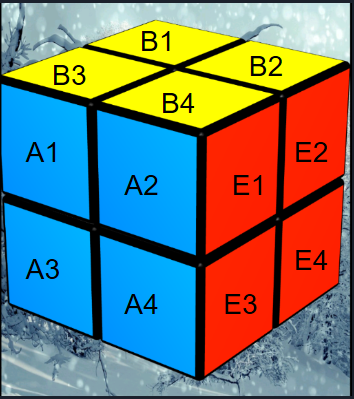
\includegraphics[width=.5\textwidth, center]{pics/Facelet.PNG} \\[7mm]
As shown in the picture, the 2x2 cube's face-lets were defined with each face receiving a designated letter (A-F) and that letter was paired with a number corresponding to the face-let position, with the number one beginning in the top left through four in the bottom left corner. It was also encoded to represent each color by an integer value. Labeling the cube in this consistent way allowed for the transitions to be reflected accurately. \\[3mm]
To accurately reflect these transitions it must be known that there are only six different moves that can be made with a standard 2x2 Rubik's Cube. \\[7mm]
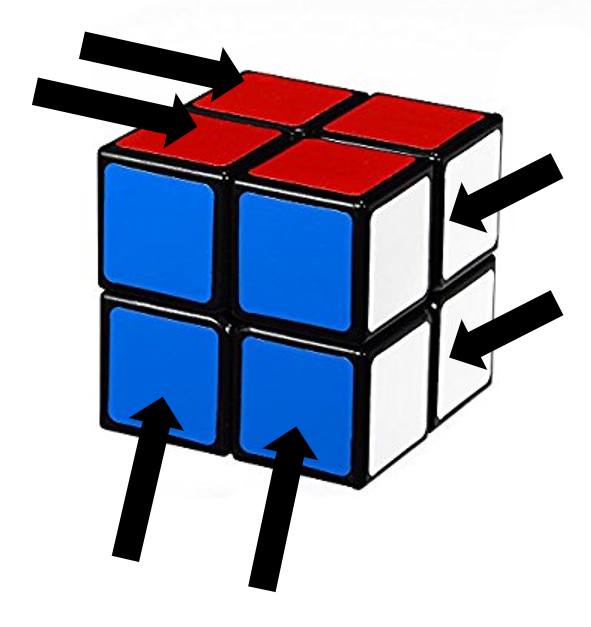
\includegraphics[width=.5\textwidth, center]{pics/Capture5} \\[7mm]
These moves, reflected above, were all set to rotate in a clockwise direction. Again, this consistency allowed for the encoded transitions to reflect the physical cube's movements. \\[3mm]
The final aspect of the cube that needed to be encoded was the final state that the program was attempting to reach. Initially, this proved to be a very messy and long LTL property due to the fact that each side could have six possible colors when the cube was solved. However, the SatRubiks team found that this issue could be cleaned up by working backwards. Meaning that instead of having an initial state be the random configuration of the cube, the initial state could be encoded to represent a solved cube and the final state would then represent the random configuration. This idea removed the need for nasty LTL properties and made made the code relatively easy to read and understand. \\[3mm]
Now that the cube has been setup accurately with Promela and the transitions have been correctly encoded, the ideas that were utilized in the initial programs are ready to be applied to the 2x2 Rubik's cube. The full Promela code for the 2x2 Rubik's cube can be found in Appendix B or on GitHub in the SatRubiks repository. \\[3mm]
It is important to note that when running this code with Spin some of the settings will have to be adjusted. For instance, when running this code the ``physical memory available'' will have to be adjusted from its default setting to that of at least 1,000,000 MB. If this setting is not adjusted it causes catastrophic errors within Spin and the program will fail to run. Another important aspect of running this code is that the search mode will need to be changed from depth-first search to breadth-first search. This will change the way that Spin searches the state-space of the cube. Instead of ``walking through'' each node one by one as it does in a depth search, Spin will search the node's nearest neighbors before moving on down the state-space tree. This significantly reduces run times. When run with the depth-first search set the program was seeing run times anywhere from 30 minutes to well over an hour. Changing this setting cut the run times down to the level of seconds to a few minutes. 
\subsection{Results}
In order to generate random configurations of a 2x2 Rubik's cube, the SatRubiks team used a popular application for the iPhone, \textit{Cube 3D Kit}. This application provided a platform that could not only generate random initial conditions but also allow the user to attempt to solve the puzzle. Using this application, several random configurations were generated and ran against the Spin model. Depending on the initial configuration of the cube the model could solve it in as little as half a second, however in some uncommon cases it could take up to a couple minutes. Below are two different configurations of the 2x2 cube that were checked against the model. \\

\begin{figure}[!h]
  \centering
  \begin{minipage}[b]{0.4\textwidth}
    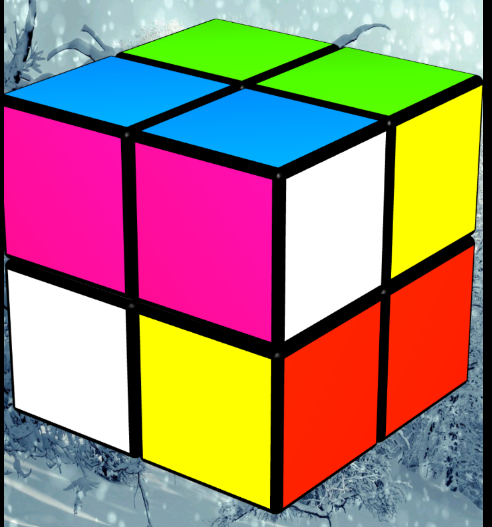
\includegraphics[width=\textwidth]{pics/Capture6.PNG}
    \caption{Random Config.A}
  \end{minipage}
  \hfill
  \begin{minipage}[b]{0.4\textwidth}
    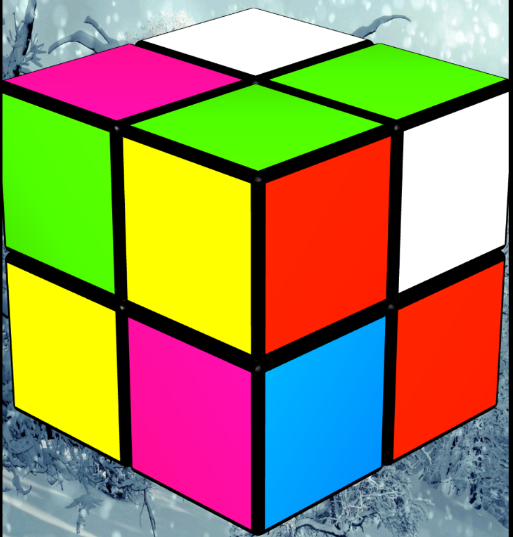
\includegraphics[width=\textwidth]{pics/Capture8.PNG}
    \caption{Random Config. B}
  \end{minipage}
\end{figure}
By inputting the appropriate orientation into the Spin model, the algorithm provided a correct path that led to the solved cube when followed in reverse. Note that each clockwise transition will now represent a counter-clockwise transition due the backward nature of the program. In the first case, the algorithm was able to solve the puzzle in just .49 seconds. Provided a path that consisted of seven moves to be solved.  The second configuration took a little longer for the algorithm to solve, solving it in 10.9 seconds. This amount of time was rather common when running other tests. Only in a few instances was there long run times of several minutes. However, there was not a lot of consistency in the run times and some instances where this model was not able to solve the initial configuration given.
\subsection{Verification and Future Work}
Attempting to make sure that the model accurately reflected the cube and its moves was one of the more difficult tasks. There was no real good way to validate the transitions aside form the use of inspection. To make this as accurate as possible, all transitions were explicitly written out including what each face-let was doing during a single rotation. These were then compared with the encoded information to ensure an that the physical cube was appropriately reflected. \\[3mm]
The model was also verified by using the way the cube is constructed and checking to see if certain configurations are allowed in the model. For instance, in the cube above yellow and white are on opposite sides of the cube and thus can never be next to each other in any configuration. By using simple LTL propositions, such as !(b3 == 2 \&\& a1 == 4) if two and four represent yellow and white receptively, this can be check to be sure that the model does 
not allow this to occur. This same principle can also be applied to trying to find paths that lead to impossible end states in our model. Running the model using a final state that represents white and yellow being next to each other the algorithm should not produce any trace that allows for this either. \\[3mm]
There is still more work needing to be done with the 2x2 model. The model should be able to solve every configuration that it is given. This could be a memory issue within Spin, it is not clear. However, expanding this model to the 3x3 cube should not be overly difficult considering how the 2x2 cube is represented and how the transitions are encoded.  The concern with this is with the memory limitations that were encountered using the Spin for the 2x2 model. 

\section{Pure SAT Solving}
\subsection{Background}
Satisfiability solving (SAT) is a method for determining the satisfying solution to a given boolean equation. SAT solving was the first problem to be determined NP-complete via the Cook-Levin theorem. Therefore, this formal method provides a unique and promising solution to the problem discussed in this paper, the Rubik's cube.
\subsection{Set-Up}
\subsubsection{Method}
In regards to solving a Rubik’s cube with formal methods, using a Satisfiability Solver (SAT) has been discussed the most throughout literature [1]. Therefore, this approach, initially, appeared to be the most straightforward of the processes discussed in this paper. This proved to be true as work started on developing the pure SAT model. With the aid of a program called Sabr [2], creating SAT queries for the Rubik’s cube became not only trivial but extremely simple. Not only were the models easy to develop but Sabr also parses the output of any given SAT solver into a format that is easy to read and follow. This allowed us to compare the efficiency of the Sabr parsing with that of NuXmv as well as the efficiency of a variety of SAT solving back ends. The overall process for solving a Rubik’s cube via SAT can be observed in figure 3: \\[7mm]
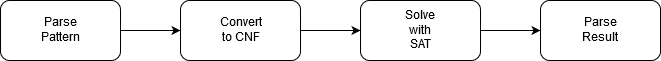
\includegraphics[width=1\textwidth, center]{pics/satfigure1.png} \\
\begin{center}
Figure 3. SAT Solving process \\[7mm]
\end{center}
\subsubsection{Parsing with Sabr}
This input to Sabr comprises of a few different main definitions: Board, Start, End, and DesObjs. With these components a model can be created as seen in model Appendix B. The initial state of an unsolved Rubik’s cube is placed in the Start definition with the following structure:\\[7mm]
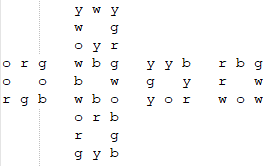
\includegraphics[width=0.5\textwidth, center]{pics/initialsabrmodel.PNG} \\
\begin{center}
Figure 4. Initial Sabr model condition \\[7mm]
\end{center}
Sabr then converts this initial condition, along with the transition definitions, into a SAT query that can be inputted into any SAT solver that utilizes the conjunctive normal form (CNF) formula structure. CNF is a form of logical equation that is constructed of ands of clauses of ors. An example of a CNF formula can be observed below where each new line is denoted with a 0 and each line is a new clause. Each variable can either be positive or negative, where negative numbers represent the negation of that variable. The first line of a CNF formula (starting with a “p”) expresses the number of variables and the number of clauses in the generated formula. These numbers were useful later in determining the correctness of the developed models because the number of variables used to solve a Rubik’s cube is known. \\
\begin{center}
p cnf 2484 23442 0 71 0 113 0 211 0 295 0 337 0 \hfill Equation 1
\end{center}
\subsubsection{SAT Solvers}
Two SAT solvers were considered during this project, the first being a SAT solver created during the 2017 SAT competition called CaDiCaL [3] and the second being the popular solver miniSat. MiniSat was chosen because of its popularity and it is also the back-end for NuXmv which allowed for another avenue of comparison between the proposed models. CaDiCaL was chosen for its performance in the agile track during the 2017 SAT solver competition. Placing first in this category showed that this was one of the quickest and simplest solvers created just recently. This created an interesting dimension to the comparison described throughout this paper.
\subsection{Results}
Initially, a 2x2 model of the Rubik’s cube was created to determine the feasibility of the proposed SAT method. What soon became obvious was that this method was very easy to work with and the results were proving to be accurate after a few test runs of the model. Only a few patterns that were tested resulted in long run times and were unable to be solved. Following the success of the 2x2 model a 3x3 model was created and analysis was performed on the results of that model as well. Unlike the 2x2 model, the 3x3 model proved to be much more difficult to get results, with most patterns running for days without a solution. This made it difficult to produce usable results from the 3x3 model, however the method was verified with the 2x2 model and the results from that are still very comparable to the other methods described in this paper.
\subsubsection{2x2 Model}
Average benchmarking results can be observed in table 1 below with extended results available in the Github source and in A1. \\
\begin{center}
Table 1. 2x2 Rubik's Cube average results \\
\begin{tabular}{|c|c|c|}
\hline
\multicolumn{3}{|c|}{2x2 Rubik's Cube} \\
\hline
& CPU Time (s) & Memory Used (Mb) \\
\hline
Sabr/miniSAT & 216.4 & 31.41 \\
\hline
CaDiCaL & 43.96* & 12.394 \\
\hline
\end{tabular} \\[0.1mm]
* Encountered runtimes $>$ 200,000 seconds
\end{center}

\subsubsection{3x3 Model}
Average benchmarking results can be observed in table 2 below with extended results available in the Github source and in A2. \\
\begin{center}
Table 2. 3x3 Rubik's Cube average results \\
\begin{tabular}{|c|c|c|}
\hline
\multicolumn{3}{|c|}{3x3 Rubik's Cube} \\
\hline
& CPU Time (s) & Memory Used (Mb) \\
\hline
Sabr/miniSAT & 5041.31 & 305.36 \\
\hline
CaDiCaL & NA & NA \\
\hline
\end{tabular}
\end{center}
\subsubsection{Verification}
The models discussed here were verified using a few different techniques. Among those are visual inspection, random testing, and intentional error introduction. Due to Sabr's simple layout and requirements determining the correctness of the input models was a non-issue just by visual inspection. This was further supported by receiving correct counterexamples that led to a valid cube solution. A variety of different patterns were also tested to guarantee that the model was producing accurate results. This was also validated by the use of different SAT solvers which allowed for the comparison of their respective outputs. Errors were also intentionally placed within the model to validate that the resulting CNF formula was not satisfiable. This was done by placing an incorrect amount of a certain color of face into the model and by putting colors that cannot physically exist next to each other. After this verification, the accuracy of the results of these models can be considered reasonably high.
\subsubsection{Conclusions}
As clear as the results shown in table 1 appear to be, the extended results shown in A1 and A2 express a different yet complicated set of data. Given the average data, one would say that CaDiCaL is the clear winner in terms of memory usage and runtime, however when looking at the efficiency of the solver itself, in terms of number of propagations, decisions, and amount minimized, the winner looks much more like miniSat. Therefore, miniSat could be considered more robust than CaDiCaL in that it solves more patterns in about the same amount of time, compared to CaDiCaL, which could solve some patterns very quickly, but others in an unreasonable amount of time. Despite the limited amount of data for the 3x3 cube this conclusion could be extrapolated to the increased level of computation. The advantage of CaDiCaL, however, is that it uses much less memory than miniSat which for systems with little memory, then CaDiCaL may be the better option. Overall, using Sabr with it's miniSat back-end is a very easy to use, accurate, and relatively efficient method for solving a Rubik's cube.
\subsubsection{Future Work}
More work needs to be done in solving the issues with the SAT solvers not being able to solve some of the patterns in a reasonable amount of time. Even the patterns that miniSat could solve, yet CaDiCaL failed, shows that there is something in CaDiCaL that may have been over looked. Unfortunately, there will always be memory issues when dealing with this immense amount of variables, but future work in making that number even smaller will only allow for a decrease in runtime and memory usage.

\newpage

\section{A Bounded Model Checking Approach}

\subsection{Background}
When model checking an incredibly large finite (or potentially infinite) state space, a natural approach consists of limiting the search to only those states that are deemed ``relevant"; in many cases, this ``relevance" may be defined by a proximity to the start of the model, a finite limit on the distance from the initial state that is to be checked. The number of steps from the initial state, $k$, that must be visited to demonstrate adherence of a system to a particular property is referred to as the \textit{completeness threshold} (CITE). For a property, such as $\always \phi$, $k$ is selected such that all states are reachable within $k$ steps from the initial state. Thus, showing that no property violation occurs in this bound is sufficient to demonstrate that no violation occurs for any valid run of the system.

\subsection {Method}
As demonstrated by (CITE) in (YEAR), the 2x2x2 Rubik's Cube is designed such that the upper bound on the number of (quarter-turn) moves between any two states is 14. This serves as a natural bound for model checking this system, as a solution to the cube must reachable within 14 moves.

\subsection {2x2x2 Model}

\subsubsection {nuXmv}

\subsubsection {C}

\subsubsection {C Bounded Model Checker (CBMC)}

\subsection {Verification}

\subsection {CBMC Results}

\subsection {3x3x3 Model}

\subsubsection {C}

\subsubsection {C Bounded Model Checker (CBMC)}

\subsection {Verification}

\subsection {Initial CBMC Results}

\subsection {"Under the hood": Minisat and CBMC}

\subsection {Revised C Model}

\subsection {Final CBMC Results}

\subsection {Conclusion}

\subsection {Future Work}

\newpage

\section{Final Conclusions}


\pagebreak
\begin{center}
Appendix A
\end{center}

\begin{center}
Table 1. Extended miniSat 2x2 Rubik's cube results \\[1mm]
\end{center}
\begin{adjustwidth}{-3.5cm}{}
\begin{tabular}{|c|c|c|c|c|c|c|c|c|c|}
\hline
Run Number & SAT & Parse time & Restarts & Conflicts /sec & Decisions /sec & Conflict literals & Memory used & CPU time \\
\hline
0 & Y & 0.01 s & 307 & 24015 & 42318 & 16.40\% deleted & 18.83 MB & 4.776 s \\
\hline
1 & Y & 0.01 s & 1341 & 21611 & 32719 & 15.89\% deleted & 25.42 MB & 29.368 s \\
\hline
2 & N & 0.01 s & 1532 & 24952 & 37551 & 23.72\% deleted & 24.79 MB & 28.036 s \\
\hline
3 & Y & 0.01 s & 2044 & 20364 & 30679 & 18.07\% deleted &  26.29 MB & 46.368 s \\
\hline
4 & Y & 0.01 s & 24574 & 13853 & 18578 & 35.33\% deleted & 80.81 MB & 1186.84 s \\
\hline
5 & Y & 0.01 s & 236 & 26659 & 44732 & 13.62\% deleted & 12.32 MB & 2.812 s \\
\hline
\end{tabular} \\[3mm]
\end{adjustwidth}

\begin{center}
Table 2. Extended CaDiCaL 2x2 Rubik's cube results \\[1mm]
\end{center}
\begin{adjustwidth}{-3.5cm}{}
\begin{tabular}{|c|c|c|c|c|c|c|c|c|c|}
\hline
Run Number & SAT & Parse time & Restarts & Conflicts /sec & Decisions /sec & Conflict literals & Memory used & CPU time \\
\hline
0 & Y & 0.01 s & 9813 & 390697 & 11103.13 & 7.63\% deleted & 15.67 MB & 35.67 s \\
\hline
1 & Y & 0.01 s & 4693 & 13438.41 & 53381.47 & 7.35\% deleted & 9.10 MB & 11.59 s \\
\hline
2 & N & 0.01 s & 3167 & 16655.43 & 57761.16 & 7.81\% deleted & 8.47 MB & 7.89 s \\
\hline
3 & Y & 0.01 s & 29175 & 5824.01 & 21442.38 & 11.11\% deleted & 21.96 MB & 160.65 s \\
\hline
4 & Y & 0.01 s & NA & NA & NA & NA & NA & $\>$ 20000 s \\
\hline
5 & Y & 0.01 s & 2172 & 18536.71 & 74321.68 & 6.05\% deleted & 6.77 MB & 4.00 s \\
\hline
\end{tabular}
\end{adjustwidth}

\pagebreak
\begin{center}
Appendix B
\end{center}
\begin{lstlisting}
/*colors: 1=blue, 2=yellow, 3= green, 4=white, 5=red, 6=pink */
byte a1=1, a2=1, a3=1, a4=1, b1=2, b2=2, b3=2, b4=2, c1=3, c2=3, c3=3, c4=3, d1=4, d2=4, d3=4, d4=4, e1=5, e2=5, e3=5, e4=5, f1=6, f2=6, f3=6, f4=6;
byte tmp1=0, tmp2=0, tmp3=0, tmp4=0, tmp5=0, tmp6=0, tmp7=0, tmp8=0, tmp9=0, tmp10=0, tmp11=0, tmp12=0;	
#define ASIDE (a1==6 && a2==6 && a3==4 && a4==2)
#define BSIDE (b1==3 && b2==3 && b3==1 && b4==1)
#define CSIDE (c1==5 && c2==5 && c3==4 && c4==2)
#define DSIDE (d1==3 && d2==1 && d3==3 && d4==1)
#define ESIDE (e1==4 && e2==2 && e3==5 && e4==5)
#define FSIDE (f1==4 && f2==2 && f3==6 && f4==6)
#define FINISH (ASIDE && BSIDE && CSIDE && DSIDE && ESIDE)
active proctype rubiks()
{
	do
	
	::assert(!FINISH) -> atomic{
		tmp1=a2;
		tmp2=a4;
		tmp3=b2;
		tmp4=b4;
		tmp5=c1;
		tmp6=c3;
		tmp7=d2;
		tmp8=d4;
		tmp9=e1;
		tmp10=e2;
		tmp11=e3;
		tmp12=e4;
		a2=tmp7;
		a4=tmp8;
		b2=tmp1;
		b4=tmp2;
		c1=tmp4;
		c3=tmp3;
		d2=tmp6;
		d4=tmp5;
		e2=tmp9;
		e4=tmp10;
		e3=tmp12;
		e1=tmp11;	
		printf("Right")
		}
	
	::assert(!FINISH)->atomic{
		tmp1=a1;
		tmp2=a3;
		tmp3=b1;
		tmp4=b3;
		tmp5=c2;
		tmp6=c4;
		tmp7=d1;
		tmp8=d3;
		tmp9=f1;
		tmp10=f2;
		tmp11=f3;
		tmp12=f4;
		a1=tmp7;
		a3=tmp8;
		b1=tmp1;
		b3=tmp2;
		c4=tmp3;
		c2=tmp4;
		d1=tmp6;
		d3=tmp5;
		f3=tmp9;
		f4=tmp11;
		f2=tmp12;
		f1=tmp10;	
		printf("Left")
		}
	
	::assert(!FINISH)->atomic{
		tmp1=a1;
		tmp2=a2;
		tmp3=e1;
		tmp4=e2;
		tmp5=c1;
		tmp6=c2;
		tmp7=f1;
		tmp8=f2;
		tmp9=b1;
		tmp10=b2;
		tmp11=b3;
		tmp12=b4;
		a1=tmp3;
		a2=tmp4;
		e1=tmp5;
		e2=tmp6;
		c1=tmp7;
		c2=tmp8;
		f1=tmp1;
		f2=tmp2;
		b2=tmp9;
		b4=tmp10;
		b3=tmp12;
		b1=tmp11;	
		printf("Top")
		}	
	
	::assert(!FINISH)->atomic{
		tmp1=a3;
		tmp2=a4;
		tmp3=e3;
		tmp4=e4;
		tmp5=c3;
		tmp6=c4;
		tmp7=f3;
		tmp8=f4;
		tmp9=d1;
		tmp10=d2;
		tmp11=d3;
		tmp12=d4;
		a3=tmp3;
		a4=tmp4;
		e3=tmp5;
		e4=tmp6;
		c3=tmp7;
		c4=tmp8;
		f3=tmp1;
		f4=tmp2;
		d4=tmp11;
		d2=tmp12;
		d1=tmp10;
		d3=tmp9;	
		printf("Bottom")
		}
	
	::assert(!FINISH)->atomic{
		tmp1=b3;
		tmp2=b4;
		tmp3=f2;
		tmp4=f4;
		tmp5=e1;
		tmp6=e3;
		tmp7=d1;
		tmp8=d2;
		tmp9=a1;
		tmp10=a2;
		tmp11=a3;
		tmp12=a4;
		b4=tmp3;
		b3=tmp4;
		d2=tmp5;
		d1=tmp6;
		f2=tmp7;
		f4=tmp8;
		a2=tmp9;
		a4=tmp10;
		a1=tmp11;
		a3=tmp12;
		printf("Front")
		}
	
	::assert(!FINISH)->atomic{
		tmp1=b1;
		tmp2=b2;
		tmp3=f1;
		tmp4=f3;
		tmp5=e2;
		tmp6=e4;
		tmp7=d3;
		tmp8=d4;
		tmp9=c1;
		tmp10=c2;
		tmp11=c3;
		tmp12=c4;
		b2=tmp3;
		b1=tmp4;
		e2=tmp1;
		e4=tmp2;
		d3=tmp6;
		d4=tmp5;
		f1=tmp7;
		f3=tmp8;
		c3=tmp9;
		c1=tmp10;
		c4=tmp11;
		c2=tmp12;
		printf("Back")
		}
	od
}
od
}

\end{lstlisting}

\begin{center}
Sabr 3x3 Rubik's Cube model
\end{center}
\begin{lstlisting}
# SABR
# solve 3x3 rubiks cube

Sym{ b o w r g y }

Board{
.....		b1 b2 b3;
.....		b4 .  b6;
.....		b7 b8 b9;
r1 r2 r3	y1 y2 y3 	o1 o2 o3	w1 w2 w3;
r4 .  r6	y4 .  y6 	o4 .  o6	w4 .  w6;
r7 r8 r9	y7 y8 y9 	o7 o8 o9	w7 w8 w9;
.....		g1 g2 g3;
.....		g4 .  g6;
.....		g7 g8 g9;
}

Start{
		y g b;
		g	g;
		o b w;
r o g	w r b	o y y	o r b;
b	w	o	b	y	b	o	w;
b w w	b y g	y r g	r o r;
		r r o;
		g	w;
		w y y;
}

End{
		b b b;
		b   b;
		b b b;
r r r	y y y 		o o o	w w w;
r   r	y   y 		o   o	w	w;
r r r	y y y 		o o o	w w w;
		g g g;
		g   g;
		g g g;
}

Trans Clock:Side{

	t1 t2 t3;

l3	f1 f2 f3	r1;
l2	f4    f6	r2;
l1	f7 f8 f9	r3;

	b1 b2 b3;
=>
	l1 l2 l3;

b1	f7 f4 f1	t1;
b2	f8    f2	t2;
b3	f9 f6 f3	t3;

	r3 r2 r1;
}

Trans CounterClock:Side{

	t1 t2 t3;

l3	f1 f2 f3	r1;
l2	f4    f6	r2;
l1	f7 f8 f9	r3;

	b1 b2 b3;
=>
	r1 r2 r3;

t3	f3 f6 f9	b3;
t2	f2    f8	b2;
t1	f1 f4 f7	b1;

	l3 l2 l1;
}

DesObj Front:Side{
	b7 b8 b9;
	
r3	y1 y2 y3	o1;
r6	y4    y6	o4;
r9	y7 y8 y9	o7;
	
	g1 g2 g3;
}

DesObj Top:Side{
	w3 w2 w1;

r1	b1 b2 b3	o3;
r2	b4    b6	o2;
r3	b7 b8 b9	o1;

	y1 y2 y3;
}

DesObj Back:Side{
	b3 b2 b1;

o3	w1 w2 w3	r1;
o6	w4    w6	r4;
o9	w7 w8 w9	r6;

	g8 g7 g6;
}

DesObj Bottom:Side{
	y7 y8 y9;

r9	g1 g2 g3	o7;
r8	g4    g6	o8;
r7	g7 g8 g9	o9;

	w9 w8 w7;
}

DesObj Left:Side{
	b1 b4 b7;

w3	r1 r2 r3	y1;
w6	r4    r6	y4;
w9	r7 r8 r9	y7;

	g7 g4 g1;
}

DesObj Right:Side{
	b9 b6 b3;

y3	o1 o2 o3	w1;
y6	o4    o6	w4;
y9	o7 o8 o9	w7;

	g3 g6 g9;
}
\end{lstlisting}

\newpage

\begin{thebibliography}{9}
\bibitem{chenjingchao} 
Chen, Jingchao. 
\textit{{Solving Rubik's Cube Using SAT Solver}. 
Computing Research Repository - CORR, 2011.}

\bibitem{sabr} 
\textit{{Sabr}. 
http://sabrlang.org/}

\bibitem{CaDiCaL} 
\textit{{CaDiCaL}. 
http://fmv.jku.at/cadical/}

\bibitem{satrubiks}
SatRubiks.
\textit{{Github repository}.
https://github.com/IowaStateAerospaceCourses-Rozier/final-project-satrubiks}
\end{thebibliography}

\end{document}
